% !TEX root = main.tex
\chapter{Theory}

\section{Bridge Weigh-in-Motion}
A Bridge Weigh-in-Motion system is based on measurements of a bridge's deformation. The BWIM system uses these measurements to calculate passing vehicles axle loads.
There are different approaches to assembling such a system, but they typically consists of a strain gauge measuring the strain induced by passing vehicles, a axle detector used to find the vehicle speed and spacing of axles and a computer or data storage device. An algorithm then is able to use the data gathered from the axle detector and strain gauge to calculate axle loads \cite{Quilligan}.
\subsection{Moses' Algorithm}
Moses' algorithm is based on the fact that a moving load along a bridge will set up stresses in proportion to the product of the value of the influence line and the axle load magnitude. The influence line being defined as the bending moment at the point of measurement due to a unit axle load crossing the bridge \cite{Quilligan}.

Moses' algorithm is built from the fact that a moving unit load on a bridge will induce stresses proportional to the product of the value of the influence line and the axle load magnitude.

Each individual girder's stress is related to moment:
\begin{equation}
\overbrace{\sigma_{i}}^\text{stress in i'th girder} = \frac{\overbrace{M_i}^\text{bending moment i'th girder}}{\underbrace{W_i}_\text{section modulus}}
\end{equation}
Expressing the moment in terms of strain gives
\begin{equation}
M_i = W_i \sigma_i = \overbrace{E}^\text{Modulus of elasticity} \times W_i \times \underbrace{\varepsilon_i}_\text{strain in i'th girder}
\end{equation}
The sum of the individual girder moments is therefore:
\begin{equation}
M = \sum_{i = 1}^{N} M_i = \sum_{i = 1}^{N} EW_i \varepsilon_i = EW \sum_{i = 1}^{N} \varepsilon_i
\label{equation:moment_strain}
\end{equation}
The sum of the girder strains is proportional to the gross bending moment. The total bending moment and the measured strain is thus directly related by $EW$. These constants can be calculated through the bridge's dimensions and material properties. However through measuring the effects of a known vehicle passing the bridge these constants can be derived.

Weigh in motion is an inverse type problem, the strain is measured and the cause of the strain is to be calculated. The theoretical bending moment corresponding to axle loads on the bridge at one strain sample, is given by:
\begin{equation}
M_k^T = \sum_{i = 1}^{N} A_i I_{(k-C_i)}
\label{equation:theoretical_strain}
\end{equation}
\begin{equation}
C_i = (L_i \times f)/v
\end{equation}
Where:
\begin{description}
	\item N = \textit{the number of vehicle axles}
	\item $A_i = $ \textit{the weight of axle i}
	\item $I_{k-C_i} = $ \textit{the influence line ordinate for axle i at sample k}
	\item $L_i$ = the distance between axle i and the first axle in meters
	\item $C_i$  = \textit{The number of strain samples corresponding to the axle distance $L_i$}
	\item f = the strain gauge's sampling frequency, in \SI{}{\Hz}
\end{description}

\section{Influence lines}
For a B-WIM system the influence line is defined as "the bending moment at the point of measurement due to a unit axle load moving along the bridge \cite{bwim_an_overview}". The influence line could be found through assembling a model of the bridge in any CAD or frame-program, this would however take a lot of time especially for more advanced bridge's. Depending on the support of the bridge the influence lines takes different theoretical forms, as seen in Figure \ref{fig:theoreticalInfl}. The true influence line for a bridge lie somewhere in between the simply supported and fixed version \cite[p.~146]{bwim_an_overview}.
Influence lines is a big source of error in a B-WIM system.
\begin{figure}[h]
\centering
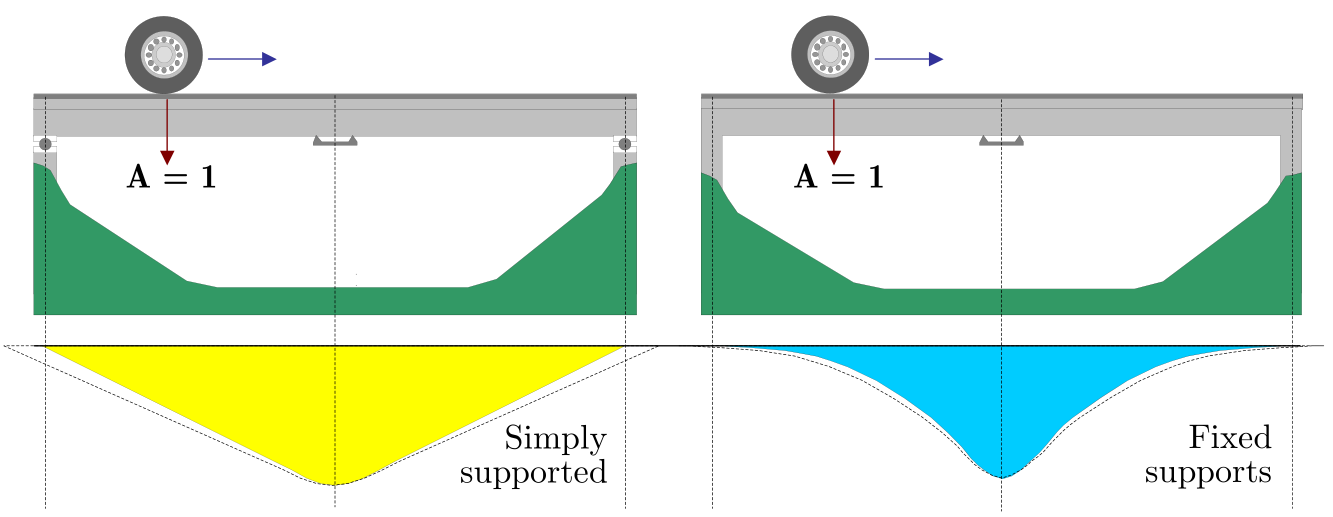
\includegraphics[scale=0.5]{figures/inflLinesQuilligan}
\caption{Influence lines for simply and fixed supported bridges, figure from \cite{Quilligan}}
\label{fig:theoreticalInfl}
\end{figure}

Znidaric and Baumgärter \cite{bwim_an_overview}, did a study on the effect of choice of influence line. This study shows errors up to 10\% for a short \SI{2}{\metre} bridge span and errors of several hundred percent for a \SI{32}{\metre} bridge span. This underlines the importance of using correct influence lines for a B-WIM system.
\begin{figure}[h]
\centering
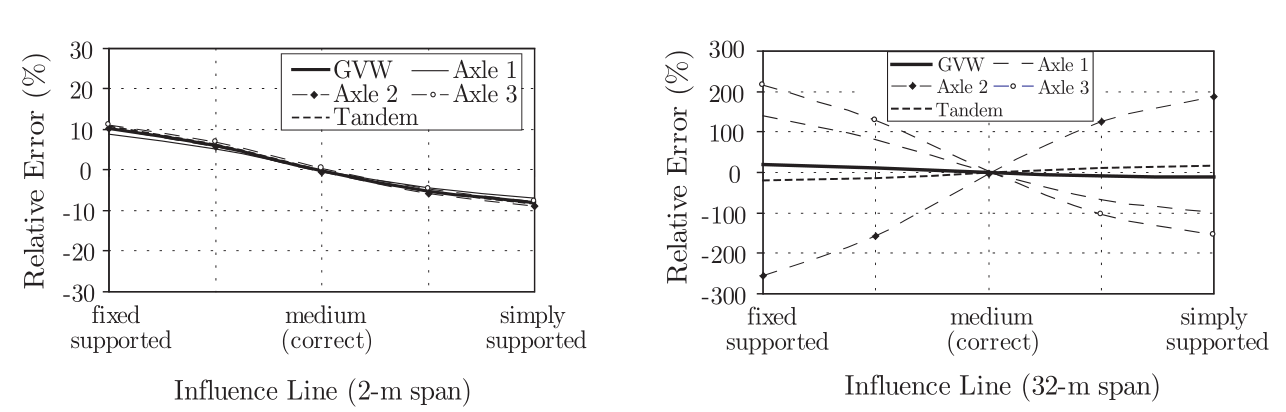
\includegraphics[scale=0.5]{figures/error_in_weights_dueTo_infl}
\caption{Errors of axle loads due to wrongly selected influence lines, figure from \cite{Quilligan}}
\label{fig:errorOfInfl}
\end{figure}

\subsection{Using influence lines, in the BWIM system}
Even if a correct influence line for a BWIM setup is found, wrong placement of the influence line with respect to the strain signal is a major source of error. In theory it should be possible to detect the excact point of a axle passing over the sensor, as it results in a peak in the strain signal. This peak corresponds to the major peak in the influence line. A good example of this is seen in figure \ref{fig:strain_vs_influenceLine}, which shows the influence line aligned with the strain signal from a 3 axle vehicle.
\begin{figure}[htbp]
	\begin{adjustbox}{center}
		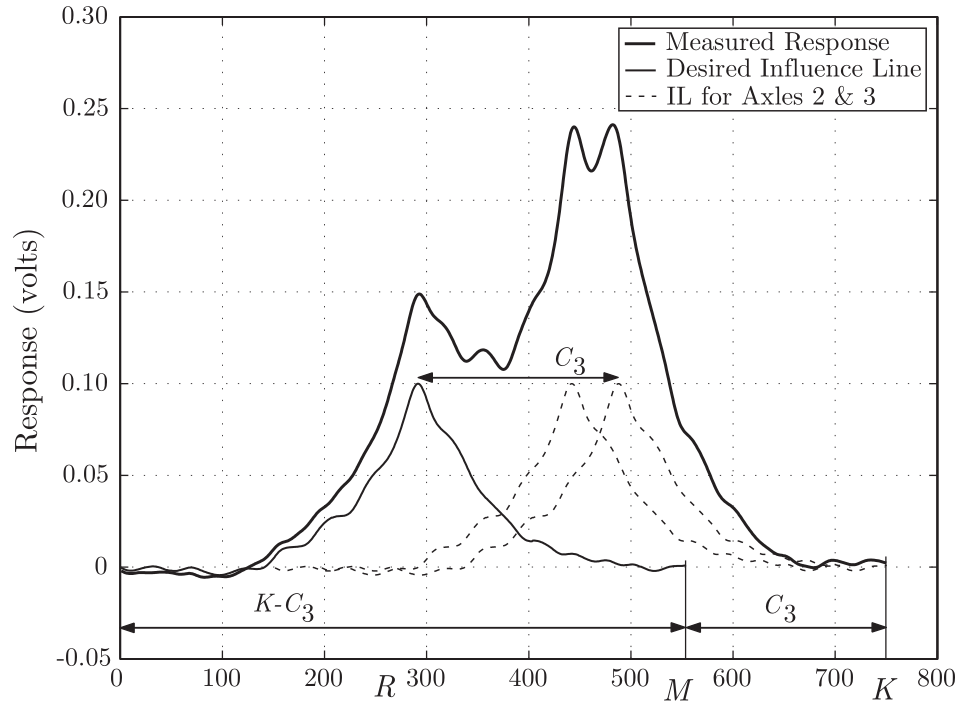
\includegraphics[width=0.9\textwidth]{figures/strain_vs_influenceline}
	\end{adjustbox}
	\caption{Placement of influence lines, influence line has been scaled.}
	\label{fig:strain_vs_influenceLine}
\end{figure}
The first peak of the strain signal corresponding to the the first axle of the vehicle should occur at the same location as the the peak of the influence line, which should be precisely at the sensor location.
For closely spaced axles it may be difficult to detect the individual peaks, because the both influence the sensor at the same time and because of system noise and dynamics.

\subsection{Matrix method}
Quilligan \cite{Quilligan} developed a 'matrix method' to calculate the influence line of a bridge through the measured strain induced by a vehicle. This method is derived from Moses', equation \ref{equation:moses}. The matrix method calculates a influence line for a specific strain signal given a known train with known axle weights and velocity. The found influence line is therefore subject to system noise and dynamics which are likely to vary from vehicle to vehicle. An averaging of a sufficient number of calculated influence lines should reduce the dynamic effects. The following description of the matrix method is an extension of Quilligans thesis "Bridge Weigh-in Motion : Development of a 2-D multi-vehicle algorithm \cite{Quilligan}", and shows the math for a general case with unlimited number of vehicle axles.
\begin{equation}
Error = \sum_{k = 1}^{K} [\varepsilon_{k}^{measured} - \varepsilon_{k}^{theoretical}]^2
\label{equation:moses}
\end{equation}
Equation \ref{equation:moses} were originally used to filter out the dynamic response of the bridge.
The theoretical strain in this equation can be expressed as a product of axle loads and influence ordinates at sampling points, see equation \ref{equation:theoretical_strain}, thus we can expand equation \ref{equation:moses}:
\begin{equation}
Error = \sum_{k = 1}^{K} \Big[\varepsilon_{k}^{measured} - \Big(\sum_{i = 1}^{N} A_i I_{(k-C_i)}\Big)\Big]^2
\label{equation:moses_expanded}
\end{equation}
The set of influence ordinates $I$ that minimizes $Error$, forms the wanted influence line.
\begin{equation}
\frac{\partial Error}{\partial I_R} = \frac{\partial \sum_{k = 1}^{K} \Big[\varepsilon_{k}^{measured} - \Big(\sum_{i = 1}^{N} A_i I_{(k-C_i)}\Big)\Big]^2}{\partial I_R}
\end{equation}
For a given number of known axle loads this equation comes down to a set of $(K - C_n)$ number of linear equations. Rearranging the equations and writing them in matrix form leads to:
\begin{equation}
\begin{bmatrix} Am \end{bmatrix}_{K-C_N, K-C_N} \begin{Bmatrix} I \end{Bmatrix}_{K-C_N, 1} = \begin{Bmatrix} M \end{Bmatrix}_{K-C_N, 1}
\label{equation:matrixForm}
\end{equation}
Where:
\begin{description}
\item $\begin{Bmatrix} M \end{Bmatrix}$ = a vector depending on axle weights and measured strain, $M_{i, 1} = \Big(\sum_{j = 1}^{N} A_j \varepsilon_{(i+C_j)}\Big)$
\item $\begin{bmatrix} Am \end{bmatrix}$ is a matrix depending only on the axle loads, defined by equation \ref{axleMatrix}.
\end{description}
\begin{equation}
\begin{bmatrix} Am \end{bmatrix} = \sum_{i = 1}^{N} \sum_{j = i}^{N} \begin{bmatrix} Am \end{bmatrix} + \big( A_i A_j  \begin{bmatrix} D \end{bmatrix}_{C_j - C_i}\big)
\label{axleMatrix}
\end{equation}
Which produces the upper triangle of the symmetric $ \begin{bmatrix} Am \end{bmatrix} $.
Where:
\begin{description}
\item $\begin{bmatrix} D \end{bmatrix}_{C_j - C_i}$ = a matrix containing only one diagonal of ones, where the diagonal is placed with an offset, $C_j - C_i$, from the center matrix diagonal.
\end{description}
Solving equation \ref{equation:matrixForm} for the influence ordinate vector gives the influence line for the strain history. This can be done through inversion of the $\begin{Bmatrix} M \end{Bmatrix}$ (equation \ref{axleMatrix}) or other numerical solutions like a Cholesky factorization. In this project this was done through Matlab's \textbackslash operator.
When the influence line and the axle spacings are known, the axle weights can be calculated by solving
\begin{equation}
	A = \begin{Bmatrix} I \end{Bmatrix} \textbackslash \epsilon
\end{equation}
\subsection{Optimization}
testing \cite{Liljencrantz}.
For this thesis one of the goals where to assess the accuracy of and optimization algorith for finding a bridges influence lines. To develope such an algorithm test strain signal where produced by a matlab script, and the algorithm developed was to find the influence line used to produce the strain signal.
In theory using optimization to identify influence lines should work well, and indeed it did for these produced theoretical strain signals.

\section{Finding the train's speed}
\label(section:trainSpeed)
\begin{easylist}[itemize]
 & By identifying peaks in the strain history for two different sensors, representing the same axle. The distance between the two sensors and the time difference between the found peaks should theoretically give a good estimate of the trains velocity.
 & Through doing cross correlation between two sensors strain history. This involves finding the phase difference, or lag, between the signals. The known distance between the strain gauges should then along with a constant, based on distance between sensors, give a reliable estimate of train velocity. INSERT PLOT OF CORRELATION AND SHOW MATHEMATICAL EQUATION DESCRIBING CROSS CORRELATION.
\end{easylist}
\section{The axle distances}

\section{Filtering and noise}
All signals are subjected to noise, which can be defined as
\begin{displayquote}
	unwanted disturbances superposed upon a useful signal that tend to obscure its information content \cite{IEEE_electronics}
\end{displayquote}
Noise in a BWIM system can be intrinsic noise, that is noise generated inside a system, and extrinsic noise which is noise generated outside the system. A train approaching the BWIM sensors may be a source of extrinsic noise.
Performing bridge weigh-in motion relies upon the information provided by the sensor signals. When the distances between axles is to be found, noise is a source of distortion which may increase error of found distance, it may also make it difficult for the program to detect the desired peaks in the signal which corresponds to the trains axles. Smoothing the signal may therefore completely necessary for a BWIM system. During the developement of the software for this thesis, several attempts on finding and using appropriate filters have been made. Matlab contains many such filter functions which can be used, such as a Butterworth and SGOLAY filters.
\subsection{Noise smoothing through fourier transformation}
The following quotation from  Matlabs: Practical Introduction to Frequency-Domain Analysis, see \cite{frequency_domain_analysis}, describes how frequency analysis can be done with Matlab.
\begin{displayquote}
	Frequency-domain analysis shows how a signal's energy is distributed over a range of frequencies. A signal can be converted between the time and frequency domains with a pair of mathematical operators called a transform. An example of this is the Fourier transorm which decoposes a function into the sim of a number of sine wave frequency components. The 'spectrum' of frequency components is the frequency domain representation of the signal. The inverse Fourier transform converts the frequency domain function back to a time function.
\end{displayquote}

Performing a fast fourier transformation in matlab on a vector signal, gives the oportunity to remove unwanted frequencies from the signal. When the signal is transformed into the frequency domain, setting all the frequencies above 30 Hz to zero and then transforming the signal back into the time domain would smooth a typical BWIM signal greatly.
